\chapter{Estado de la cuestión}
\label{chap:estado_cuestion}

\section{Modelos de IA generativa aplicados a la música}

En la actualidad, la generación de música o, en un sentido ámplio, de sonido, constituye uno de los frentes de investigación activos y más prometedores en el campo de la IA. La generación música con modelos de \textit{Deep Learning} ha sido abordado históricamente desde dos grandes perspectivas en función de la naturaleza de los datos generados por los modelos: la generación de música simbólica y la generación de música con audio. La primera de ellas consiste en la creación de elementos musicales como notas, acordes, melodías, etc. en un formato simbólico, ya sea MIDI, OSC, MusicXML, ABC, Lilypond, o cualquier formato musical reducible a símbolos textuales. La segunda, en la creación de un flujo de audio directamente reproducible sin necesidad de síntesis sonora o utilización de bibliotecas de \textit{samples}.

La primera aproximación, la de la composición informática de música a través de elementos simbólicos, se remonta a los inicios de la computación, con pioneros como Lejaren Hiller y Leonard Isaacson, que en 1957 crearon \textit{Illiac Suite} \citep{arizaTwoPioneeringProjects2011,funkMusicalSuiteComposed2018}, la primera composición musical generada por ordenador. Desde entonces, la generación de música simbólica ha sido abordada desde diferentes perspectivas, como la generación de música aleatoria, la generación de música a partir de reglas, la generación de música a partir de modelos probabilísticos como las cadenas de Markov, música basada en mátemática fractal, estocástica, etc. \citep{hernandez-olivanSurveyArtificialIntelligence2022}. 

La generación de audio por medio de modelos de \textit{Deep Learning} es un campo de investigación más reciente debido en parte a su gran demanda computacional, que ha estado fuera del alcance de investigadores y empresas hasta la última década. Actualmente, modelos como \textit{MuseNet}  \citep{departmentofcomputersciencesrminstituteofscienceandtechnologychennaiindia.MusenetMusicGeneration2020a}, \textit{Jukebox} \citep{dhariwalJukeboxGenerativeModel2020}, \textit{Stable Audio} \cite{StableAudioFast}, o \textit{Suno} \citep{SunoAI}, entre otros, están consiguiendo diariamente inéditos avances en lo que se refiere a la generación de música en formato de audio de una alta calidad, y, al igual que está ocurriendo con modelos de generación de imagen o vídeo, se espera que en los próximos años se produzcan avances muy significativos en este campo. 


\section{LLM asistentes para la creación de música simbólica}
\label{sec:llm_asistentes_creacion_codigo_programacion}

La aproximación a la generación de música a través de elementos simbólicos en lugar de puro audio adquiere una renovada fuerza por la aparición de los grandes modelos de lenguaje, los cuales se basan en la arquitectura \textit{Transformer}, aparecida en 2017 \citep{vaswaniAttentionAllYou2017}, por lo que es un tema de investigación muy reciente y al que se le está prestando menos atención. El grueso de las investigaciones candentes en este momento se están centrando en la generación de audio, campo más prometedor desde el punto de vista comercial. No obstante, existen recientes investigaciones en este campo, como \textit{MuseCoco} \citep{luMuseCocoGeneratingSymbolic2023}, que propone un procedimiento en dos etapas desde el input de texto en lenguaje natural del usuario hasta la generación de música simbólica en forma de partitura. La Figura \ref{fig:musecoco} muestra el esquema de funcionamiento de este sistema. 

\begin{figure}[H]
    \caption[Esquema de funcionamiento en dos pasos de MuseCoco texto--música]{Esquema de funcionamiento en dos pasos de MuseCoco en la generación de música simbólica desde texto}
    \centering
    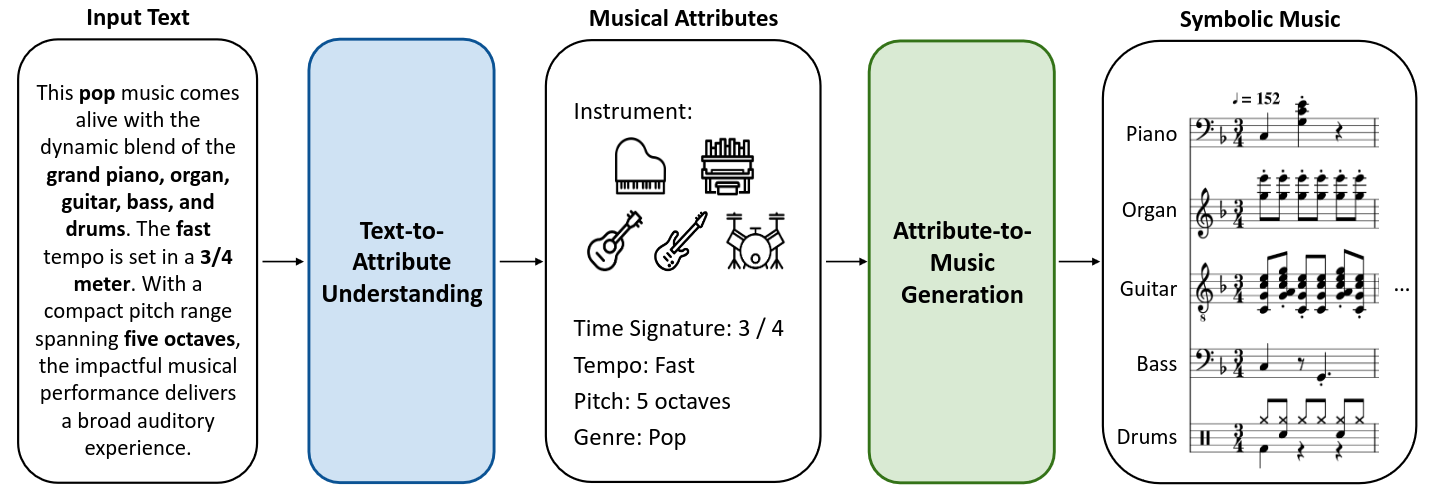
\includegraphics[width=0.9\textwidth]{./figuras/musecoco_two_steps.png}
    \source{\cite{luMuseCocoGeneratingSymbolic2023}}
    \label{fig:musecoco}
\end{figure}

Otro interesante trabajo sobre el uso de LLM para la generación musical es \textit{WavJourney} \citep{liuWavJourneyCompositionalAudio2023}, donde el papel del LLM es el de agente compositivo capaz de conectarse con otros modelos de generación de audio (voz, instrumentos, ruidos, música, etc.) para <<componer>> a partir del input o prompt del usuario. En este caso, el LLM juega un papel de mediador y planificador de la composición, además de generador de prompts para los diversos modelos implicados en la generación de audio. La Figura \ref{fig:wavjourney} muestra el esquema de funcionamiento de este sistema.

\begin{figure}[H]
    \caption[Esquema de funcionamiento de WavJourney]{Esquema de funcionamiento de WavJourney en la generación de audio desde texto}
    \centering
    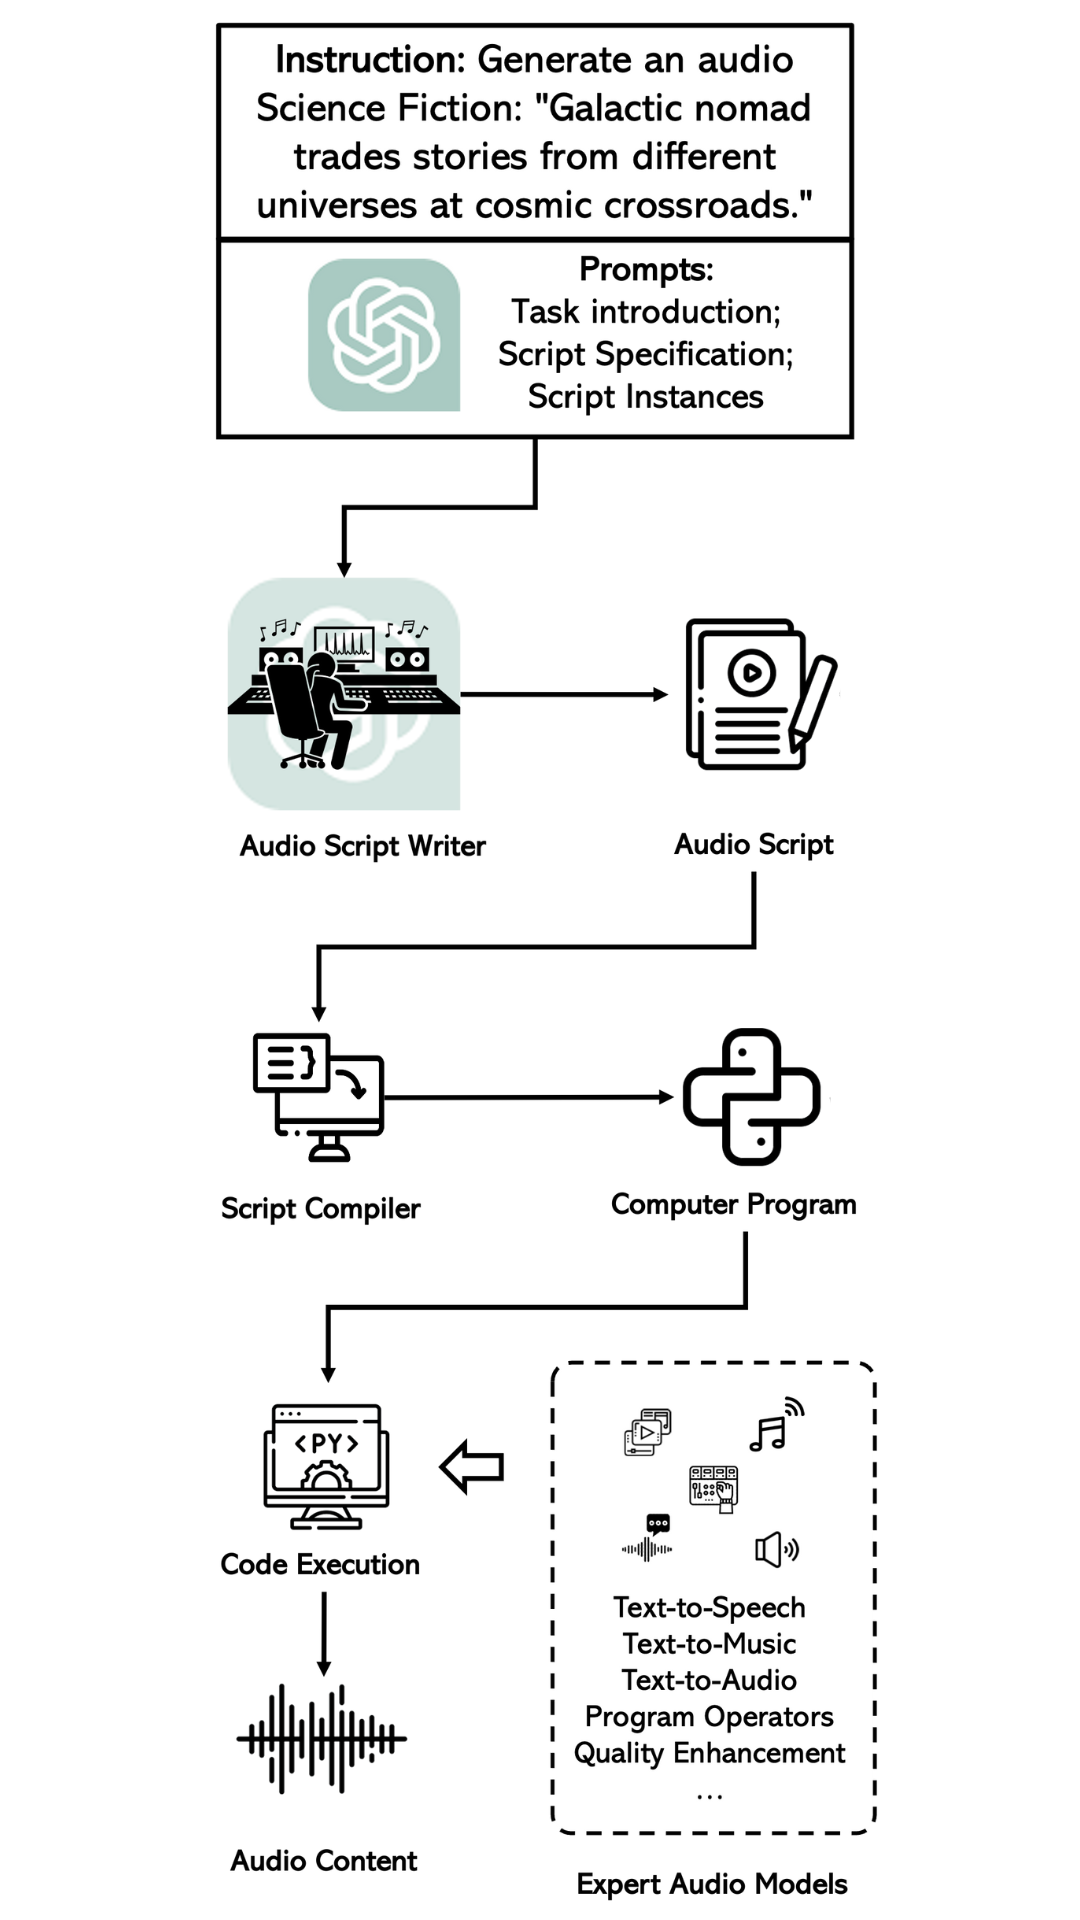
\includegraphics[width=0.4\textwidth]{./figuras/WavJourney.png}
    \source{\cite{liuWavJourneyCompositionalAudio2023}}
    \label{fig:wavjourney}
\end{figure}


La generación de código de programación por LLM, independientemente de su finalidad artística o técnica, sí que es un campo muy estudiado en los últimos meses, y que ha dado lugar a la aparición de modelos como \textit{Github Copilot}, que ha sido capaz de generar código de programación de considerable calidad a partir de inputs o \textit{prompts} en lenguaje natural. \textit{Github Copilot} es un servicio que integra un modelo GPT-4 junto a un conjunto de aplicaciones de integración en entornos de desarrollo como Visual Studio Code, Atom, etc. Debido a su amplia aplicación en el campo de la programación, es un modelo que ha recibido una gran atención mediática, y que ha sido objeto de numerosos estudios y análisis, por lo que podemos considerarlo como el estado del arte en la generación de código de programación por LLM. Es por ello que los principales estudios sobre la interacción de LLM con humanos en el campo de la programación se han centrado en este servicio. De todos estos artículos podemos extraer conclusiones de interés.

Un estudio sobre el impacto en la productividad del uso de AI en tareas concretas de programación mostró que estas se realizaron un 55,8\% más rápido que sin su ayuda \citep{pengImpactAIDeveloper2023a}, aunque necesario señalar que en este estudio participaron investigadores de Microsoft, empresa que desarrolla \textit{Github Copilot}, con lo cual los resultados pueden estar sesgados. En esta línea, investigadores Montreal y Toronto, observaron que herramientas como \textit{Github Copilot} dan resultados muy comparables a los de programadores humanos, si bien su utilidad es mayor cuando lo utilizan programadores con experiencia, constituyendo cierto riesgo en manos de programadores noveles \citep{moradidakhelGitHubCopilotAI2023}. Otro interesante estudio sobre la fiabilidad de la generación de código de \textit{Github Copilot} \citep{mastropaoloRobustnessCodeGeneration2023}, halló que en casi la mitad de los casos, el código generado por dos descripciones en lenguaje natural semánticamente equivalentes, era diferente, y en más de una cuarta parte de los casos la corrección del código se vio comprometida, lo que pone en tela juicio la robustez del sistema.

\section{\textit{Prompting engineering}}

Se entiende por \textit{prompting} a la forma en la que se le pide a un LLM que genere un texto. El \textit{prompt} es el texto en lenguaje natural que el usuario presenta al LLM como input. El \textit{prompting} es un campo de investigación muy activo en la actualidad, y que ha dado lugar a numerosos estudios y publicaciones. El buen desempeño de los LLM en tareas de código de programación lleva a estudios como \cite{liStructuredChainofThoughtPrompting2023}, que propone un sistema de prompting que pide al LLM una reflexión explícita sobre la implementación a realizar, en una especie de pseudocódigo, que en un segundo paso será traducido al código final de programación. Este sistema de prompting se basa en la idea de que el LLM generará código de mayor calidad si se le permite <<pensar>> la respuesta antes de generarla. En este sentido, existen sobradas publicaciones que ponen de relieve la sensibilidad de los LLM a la forma en la que le pedimos que procese la información (\textit{prompting}) y la correlación en la calidad de sus resultados \citep{zhouLeasttoMostPromptingEnables2023,weiChainofThoughtPromptingElicits2023,LLMPromptingGuide}.
 
\section{\textit{Retrieval-Augmented Generation} (RAG)}

Una de las técnicas más potentes para la generación de código, que combina la recuperación de información con la generación de texto. También de OpenAI Assistant, que ha presentado en el Keynote de 2023. \cite{WhatRetrievalaugmentedGeneration2021} y \cite{lewisRetrievalAugmentedGenerationKnowledgeIntensive2021}

% \begin{itemize}
%     \item Modelos de IA generativa aplicados a la música.
%     \item LLM asistentes para la creación de código de programación.
%     \item Lenguajes de programación musical.
%     \item Prompting engineering.
%     \item LLM y música (MIDI y otras representaciones).
%     \item LLM y música con lenguajes de programación.
% \end{itemize}


    \begin{figure}[H]
        \caption{Habilidades de los \textit{Foundation Models} de OpenAI.}
        \centering
        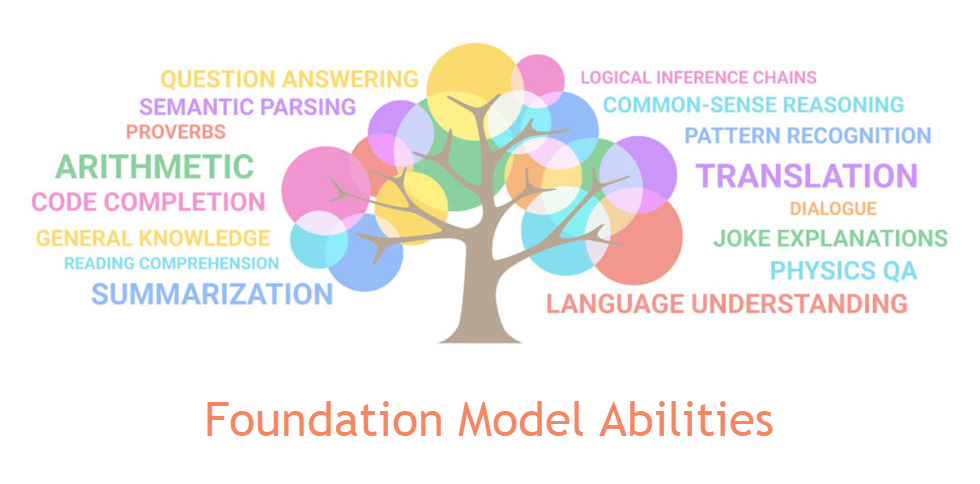
\includegraphics[width=0.8\textwidth]{./figuras/fundation_models_habilities.png}
        \source{\cite{GPT3RiseFoundation}}
        \label{fig:fundation_models_habilities}
    \end{figure}

% \section{Lenguajes de programación musical}
%     Lenguajes a modo de código de programación, como Overtone, Pure Data, Sonic Pi, Supercollider, Max MSP. Representaciones musicales susceptibles de ser generadas por LLM, como el MIDI, MusicXML, ABC, Lilypond, etc.


%     Un repaso por los papers más significativos y actuales sobre esta cuestión, especialmente las que implican la generación de código.



% \section{LLM y música (MIDI y otras representaciones) y el problema del significado}
%     Quiero exponer la distancia que supone conocer un lenguaje y usarlo para crear arte con él. Que un sistema (o un ser humano) conozca la sintaxis de un lenguaje no significa que pueda crear con él obras de arte... al menos si no se le entrena con suficientes datos.
    
%     Usar como bibliografía: el paper \cite{lewisRetrievalAugmentedGenerationKnowledgeIntensive2021} y la web \cite{WhatRetrievalaugmentedGeneration2021}

% \section{LLM y música en SuperCollider}